% Options for packages loaded elsewhere
\PassOptionsToPackage{unicode}{hyperref}
\PassOptionsToPackage{hyphens}{url}
\PassOptionsToPackage{dvipsnames,svgnames,x11names}{xcolor}
%
\documentclass[
  a4paper,
  oneside]{ETH-thesis-template}

\usepackage{amsmath,amssymb}
\usepackage{iftex}
\ifPDFTeX
  \usepackage[T1]{fontenc}
  \usepackage[utf8]{inputenc}
  \usepackage{textcomp} % provide euro and other symbols
\else % if luatex or xetex
  \usepackage{unicode-math}
  \defaultfontfeatures{Scale=MatchLowercase}
  \defaultfontfeatures[\rmfamily]{Ligatures=TeX,Scale=1}
\fi
\usepackage{lmodern}
\ifPDFTeX\else  
    % xetex/luatex font selection
\fi
% Use upquote if available, for straight quotes in verbatim environments
\IfFileExists{upquote.sty}{\usepackage{upquote}}{}
\IfFileExists{microtype.sty}{% use microtype if available
  \usepackage[]{microtype}
  \UseMicrotypeSet[protrusion]{basicmath} % disable protrusion for tt fonts
}{}
\makeatletter
\@ifundefined{KOMAClassName}{% if non-KOMA class
  \IfFileExists{parskip.sty}{%
    \usepackage{parskip}
  }{% else
    \setlength{\parindent}{0pt}
    \setlength{\parskip}{6pt plus 2pt minus 1pt}}
}{% if KOMA class
  \KOMAoptions{parskip=half}}
\makeatother
\usepackage{xcolor}
\setlength{\emergencystretch}{3em} % prevent overfull lines
\setcounter{secnumdepth}{3}
% Make \paragraph and \subparagraph free-standing
\makeatletter
\ifx\paragraph\undefined\else
  \let\oldparagraph\paragraph
  \renewcommand{\paragraph}{
    \@ifstar
      \xxxParagraphStar
      \xxxParagraphNoStar
  }
  \newcommand{\xxxParagraphStar}[1]{\oldparagraph*{#1}\mbox{}}
  \newcommand{\xxxParagraphNoStar}[1]{\oldparagraph{#1}\mbox{}}
\fi
\ifx\subparagraph\undefined\else
  \let\oldsubparagraph\subparagraph
  \renewcommand{\subparagraph}{
    \@ifstar
      \xxxSubParagraphStar
      \xxxSubParagraphNoStar
  }
  \newcommand{\xxxSubParagraphStar}[1]{\oldsubparagraph*{#1}\mbox{}}
  \newcommand{\xxxSubParagraphNoStar}[1]{\oldsubparagraph{#1}\mbox{}}
\fi
\makeatother

\providecommand{\tightlist}{%
  \setlength{\itemsep}{0pt}\setlength{\parskip}{0pt}}\usepackage{longtable,booktabs,array}
\usepackage{calc} % for calculating minipage widths
% Correct order of tables after \paragraph or \subparagraph
\usepackage{etoolbox}
\makeatletter
\patchcmd\longtable{\par}{\if@noskipsec\mbox{}\fi\par}{}{}
\makeatother
% Allow footnotes in longtable head/foot
\IfFileExists{footnotehyper.sty}{\usepackage{footnotehyper}}{\usepackage{footnote}}
\makesavenoteenv{longtable}
\usepackage{graphicx}
\makeatletter
\newsavebox\pandoc@box
\newcommand*\pandocbounded[1]{% scales image to fit in text height/width
  \sbox\pandoc@box{#1}%
  \Gscale@div\@tempa{\textheight}{\dimexpr\ht\pandoc@box+\dp\pandoc@box\relax}%
  \Gscale@div\@tempb{\linewidth}{\wd\pandoc@box}%
  \ifdim\@tempb\p@<\@tempa\p@\let\@tempa\@tempb\fi% select the smaller of both
  \ifdim\@tempa\p@<\p@\scalebox{\@tempa}{\usebox\pandoc@box}%
  \else\usebox{\pandoc@box}%
  \fi%
}
% Set default figure placement to htbp
\def\fps@figure{htbp}
\makeatother

% TODO: Add custom LaTeX header directives here

%% The following are packages that are used by the template and that you will likely need for your content. Do not change this.
\usepackage[utf8]{inputenc}
\usepackage[greek, english]{babel}
% \usepackage{CormorantGaramond}
\usepackage{hologo}
% \usepackage{natbib}
% \citestyle{aysep={,}}
\usepackage{graphicx}
\usepackage{float}
\usepackage{setspace}
\usepackage{url}
\usepackage[nottoc]{tocbibind}
\usepackage{enumitem}
\usepackage{subcaption}
\usepackage{siunitx}
\usepackage{lscape}
\usepackage{textgreek}
\usepackage{makecell}
% \usepackage[table,xcdraw]{xcolor}
% \usepackage{threeparttable}
% \usepackage{booktabs}
% \usepackage{multirow}
%\usepackage{tabularx}
\usepackage{array}
\newcolumntype{C}[1]{>{\centering\arraybackslash}m{#1}}

%% Under this line, you can add additional packages that you may need for typesetting your document.

% change spacing of bibliography entries
\usepackage[style= authoryear,
maxcitenames= 2,
maxbibnames= 999,
giveninits = false,
uniquename=false,
uniquelist=false
]{biblatex}
\setlength\bibitemsep{0.5\baselineskip}
% \setlength\bibitemsep{1.5\itemsep} % double space between references

%\usepackage{...}
\usepackage{listings}

% set up a new column type for centered columns of fixed width in latex tables
\usepackage{array}



% Set numbering of figures and tables in appendix back to 0 with each section
\usepackage{chngcntr}

%New colors defined below
\definecolor{codegreen}{rgb}{0,0.6,0}
\definecolor{codegray}{rgb}{0.5,0.5,0.5}
\definecolor{codepurple}{rgb}{0.58,0,0.82}
\definecolor{backcolour}{rgb}{0.98,0.98,0.98}

%Code listing style named "mystyle"
\lstdefinestyle{mystyle}{
  backgroundcolor=\color{backcolour}, commentstyle=\color{codegreen},
  keywordstyle=\color{magenta},
  numberstyle=\tiny\color{codegray},
  stringstyle=\color{codepurple},
  basicstyle=\ttfamily\footnotesize\tiny,
  breakatwhitespace=false,         
  breaklines=true,                 
  captionpos=b,                    
  keepspaces=true,                 
  numbers=left,                    
  numbersep=5pt,                  
  showspaces=false,                
  showstringspaces=false,
  showtabs=false,                  
  tabsize=2
}
%define Javascript language
\lstdefinelanguage{JavaScript}{
keywords={typeof, new, true, false, catch, function, return, null, catch, switch, var, if, in, while, do, else, case, break},
keywordstyle=\color{blue}\bfseries,
ndkeywords={class, export, boolean, throw, implements, import, this},
ndkeywordstyle=\color{darkgray}\bfseries,
identifierstyle=\color{black},
sensitive=false,
comment=[l]{//},
morecomment=[s]{/*}{*/},
commentstyle=\color{purple}\ttfamily,
stringstyle=\color{red}\ttfamily,
morestring=[b]',
morestring=[b]"
}
%"mystyle" code listing set
\lstset{style=mystyle}

%% Use some custom fonts
\setsansfont{FiraSans}[
    Path=fonts/,
    Scale=0.9,
    Extension = .ttf,
    UprightFont=*-Regular,
    BoldFont=*-Bold,
    ItalicFont=*-Italic,
    ]

\setmainfont{FiraSans}[
    Path=fonts/,
    Scale=0.9,
    Extension = .ttf,
    UprightFont=*-Regular,
    BoldFont=*-Bold,
    ItalicFont=*-Italic,
    ]
    
% \setmathfont{FiraMath}
    
\usepackage{quotchap} 
	% To put nice quotes at the beginning of the chapters
	
% Define colours to be used 	
\usepackage{xcolor}
\definecolor{mylightgreen}{HTML}{AACABF}
\definecolor{mydarkgreen}{HTML}{335348}
\definecolor{lightgrey}{RGB}{150,150,150}
\colorlet{chaptergrey}{mydarkgreen}
\renewcommand*{\chapnumfont}{%
  \sectfont\fontsize{120}{150}\selectfont% Default: 100/130
  \color{chaptergrey}%
  }

% Use credits package to generate a visualisation of author credits for each paper
\usepackage[role = mydarkgreen, grid = lightgrey, skipempty]{./LaTeX_pkgs/credits}

% function to control landscape page set up, currently setting page number at bottom of page and removing header
% but this approach doesn't work well for multiple page figures and, depending on size, the page number will overlap figure title 
\fancypagestyle{mylandscape}{
\fancyhf{} %Clears the header/footer
\fancyfoot{% Footer
\makebox[\textwidth][r]{% Right
  \rlap{\hspace{.75cm}% Push out of margin by \footskip
    \smash{% Remove vertical height
      \raisebox{4.87in}{% Raise vertically
        \rotatebox{90}{\thepage}}}}}}% Rotate counter-clockwise
\renewcommand{\headrulewidth}{0pt}% No header rule
\renewcommand{\footrulewidth}{0pt}% No footer rule
}

%%%%%%%%%%%%%%%%%%%%%%%%%%%%%%%%%%%%%%%%%%%%%%%%%%%%%%%%%%%%%%%%%%%%%%%%%%%%%%%%%%%%%%%%%%%%%%%%%%%%%%%%%%%%%%%%
%% The following says that all graphics (e.g. jpg, png, etc. files) will be searched in the "Figures/" folder. 
%% Do not change it but ensure you put your figures in that folder.

\usepackage{booktabs}
\usepackage{longtable}
\usepackage{array}
\usepackage{multirow}
\usepackage{wrapfig}
\usepackage{float}
\usepackage{colortbl}
\usepackage{pdflscape}
\usepackage{tabu}
\usepackage{threeparttable}
\usepackage{threeparttablex}
\usepackage[normalem]{ulem}
\usepackage{makecell}
\usepackage{xcolor}
\makeatletter
\@ifpackageloaded{tcolorbox}{}{\usepackage[skins,breakable]{tcolorbox}}
\@ifpackageloaded{fontawesome5}{}{\usepackage{fontawesome5}}
\definecolor{quarto-callout-color}{HTML}{909090}
\definecolor{quarto-callout-note-color}{HTML}{0758E5}
\definecolor{quarto-callout-important-color}{HTML}{CC1914}
\definecolor{quarto-callout-warning-color}{HTML}{EB9113}
\definecolor{quarto-callout-tip-color}{HTML}{00A047}
\definecolor{quarto-callout-caution-color}{HTML}{FC5300}
\definecolor{quarto-callout-color-frame}{HTML}{acacac}
\definecolor{quarto-callout-note-color-frame}{HTML}{4582ec}
\definecolor{quarto-callout-important-color-frame}{HTML}{d9534f}
\definecolor{quarto-callout-warning-color-frame}{HTML}{f0ad4e}
\definecolor{quarto-callout-tip-color-frame}{HTML}{02b875}
\definecolor{quarto-callout-caution-color-frame}{HTML}{fd7e14}
\makeatother
\makeatletter
\@ifpackageloaded{bookmark}{}{\usepackage{bookmark}}
\makeatother
\makeatletter
\@ifpackageloaded{caption}{}{\usepackage{caption}}
\AtBeginDocument{%
\ifdefined\contentsname
  \renewcommand*\contentsname{Table of contents}
\else
  \newcommand\contentsname{Table of contents}
\fi
\ifdefined\listfigurename
  \renewcommand*\listfigurename{List of Figures}
\else
  \newcommand\listfigurename{List of Figures}
\fi
\ifdefined\listtablename
  \renewcommand*\listtablename{List of Tables}
\else
  \newcommand\listtablename{List of Tables}
\fi
\ifdefined\figurename
  \renewcommand*\figurename{Figure}
\else
  \newcommand\figurename{Figure}
\fi
\ifdefined\tablename
  \renewcommand*\tablename{Table}
\else
  \newcommand\tablename{Table}
\fi
}
\@ifpackageloaded{float}{}{\usepackage{float}}
\floatstyle{ruled}
\@ifundefined{c@chapter}{\newfloat{codelisting}{h}{lop}}{\newfloat{codelisting}{h}{lop}[chapter]}
\floatname{codelisting}{Listing}
\newcommand*\listoflistings{\listof{codelisting}{List of Listings}}
\makeatother
\makeatletter
\makeatother
\makeatletter
\@ifpackageloaded{caption}{}{\usepackage{caption}}
\@ifpackageloaded{subcaption}{}{\usepackage{subcaption}}
\makeatother

\usepackage{hyphenat}
\usepackage{ifthen}
\usepackage{calc}
\usepackage{calculator}



\usepackage{graphicx}
\usepackage{geometry}
\usepackage{afterpage}
\usepackage{tikz}
\usetikzlibrary{calc}
\usetikzlibrary{fadings}
\usepackage[pagecolor=none]{pagecolor}


% Set the titlepage font families







% Set the coverpage font families
\usepackage{fontspec}
\newfontfamily{\coverpagetitlefont}{FiraSans-Bold.ttf}
\usepackage{fontspec}
\newfontfamily{\coverpagefooterfont}{FiraSans-Regular.ttf}


\usepackage[style= authoryear,maxcitenames= 2,maxbibnames=
999,giveninits = false,uniquename=false,uniquelist=false]{biblatex}
\addbibresource{bibliography.bib}
\usepackage{bookmark}

\IfFileExists{xurl.sty}{\usepackage{xurl}}{} % add URL line breaks if available
\urlstyle{same} % disable monospaced font for URLs
\hypersetup{
  colorlinks=true,
  linkcolor={mydarkgreen},
  filecolor={mydarkgreen},
  citecolor={mydarkgreen},
  urlcolor={mydarkgreen},
  pdfcreator={LaTeX via pandoc}}


%%%%% THESIS / TITLE PAGE INFORMATION
% Declare title pages variables so they can be specificed in _quarto.yml:
\title{Your thesis title} % Thesis title
\author{Jane Doe} % Your name
\DissNumber{XXXX} % ETH dissertation number
\degree{DOCTOR OF SCIENCES} % Your full degree name.
\degreedate{2025} % Year of degree submission
\MSctitle{Environmental Policy, Science and
Management} % Title of your MSc degree
\MScuni{Central European University, University of Manchester,
University of Lund, University of the
Aegean} % University/ies of your MSc
\citizenship{My home country} % country of birth
\dob{September 14, 1993} % date of birth
\examiner{Prof.~Dr.~Dwayne
Johnson} % Your examiner (title and name: Prof. Dr. X)
\coexaminerone{Prof.~Dr.~Stevie
Irwin} % Your 1st co-examiner (title and name: Prof. Dr. X)
\coexaminertwo{Dr.~Brian
Gumble} % Your 2nd co-examiner (title and name: Prof. Dr. X)
\summarytitle{Zusammenfassung} % Title of your tranlsated summary

% Change the colour of quarto callout boxes needs to be hear so that it is
% passed aftert the quarto default callout boxes are defined.
\colorlet{quarto-callout-note-color-frame}{mydarkgreen}
\colorlet{quarto-callout-note-color}{mydarkgreen}
\begin{document}
%%%%% CHOOSE YOUR LINE SPACING HERE
% This is approx. 1.5 spacing:
\setlength{\textbaselineskip}{18pt plus2pt minus1pt}

% You can set the spacing here for the roman-numbered pages (acknowledgements, table of contents, etc.)
\setlength{\frontmatterbaselineskip}{18pt plus2pt minus1pt}

% Leave this line alone; it gets things started for the real document.
\setlength{\baselineskip}{\textbaselineskip}

%%%%% CHOOSE YOUR SECTION NUMBERING DEPTH HERE
% You have two choices.  First, how far down are sections numbered?  (Below that, they're named but
% don't get numbers.)  Second, what level of section appears in the table of contents?  These don't have
% to match: you can have numbered sections that don't show up in the ToC, or unnumbered sections that
% do.  Throughout, 0 = chapter; 1 = section; 2 = subsection; 3 = subsubsection, 4 = paragraph...

% The level that gets a number:
\setcounter{secnumdepth}{3}
% The level that shows up in the ToC:
\setcounter{tocdepth}{2}

%%%%% begin titlepage extension code


\begin{titlepage}
% This is a combination of Pandoc templating and LaTeX
% Pandoc templating https://pandoc.org/MANUAL.html#templates
% See the README for help

\thispagestyle{empty}

\newgeometry{top=-100in}

% Page color

\newcommand{\coverauthorstyle}[1]{{#1}}

\begin{tikzpicture}[remember picture, overlay, inner sep=0pt, outer sep=0pt]

\tikzfading[name=fadeout, inner color=transparent!0,outer color=transparent!100]
\tikzfading[name=fadein, inner color=transparent!100,outer color=transparent!0]
\node[ scope fading=north, anchor=south west, rotate=0.0, opacity=0.8] at ($(current page.south west)+(0.0, 0.0)$) {
\includegraphics[width=\paperwidth, keepaspectratio]{frontmatter/images/cover\_background.png}};

% Title
\newcommand{\titlelocationleft}{18cm}
\newcommand{\titlelocationbottom}{27cm}
\newcommand{\titlealign}{right}

\begin{scope}{%
\fontsize{24}{28.799999999999997}\selectfont
\coverpagetitlefont
\node[anchor=north
east, align=right, rotate=0] (Title1) at ($(current page.south west)+(\titlelocationleft,\titlelocationbottom)$)  [text width = 20cm]  {\textcolor{mydarkgreen}{\nohyphens{Title}}};
}
\end{scope}

% Footer
\newcommand{\footerlocationleft}{18cm}
\newcommand{\footerlocationbottom}{25cm}
\newcommand{\footerlocationalign}{right}

\begin{scope}
{%
\fontsize{20}{24.0}\selectfont
 \coverpagefooterfont
\node[anchor=north east, align=right, rotate=0] (Footer1) at %
($(current page.south west)+(\footerlocationleft,\footerlocationbottom)$)  [text width = 20cm]  {\textcolor{mydarkgreen}{\nohyphens{Subtitle}}};
}
\end{scope}

\end{tikzpicture}
\clearpage
\restoregeometry
%%% TITLE PAGE START

% Set up alignment commands
%Page
\newcommand{\titlepagepagealign}{
\ifthenelse{\equal{left}{right}}{\raggedleft}{}
\ifthenelse{\equal{left}{center}}{\centering}{}
\ifthenelse{\equal{left}{left}}{\raggedright}{}
}


\newcommand{\titleandsubtitle}{
% Title and subtitle
}
\newcommand{\titlepagetitleblock}{
\titleandsubtitle
}

\newcommand{\authorstyle}[1]{{#1}}

\newcommand{\affiliationstyle}[1]{{#1}}

\newcommand{\titlepageauthorblock}{
{\authorstyle{}}}

\newcommand{\titlepageaffiliationblock}{
\hangindent=1em
\hangafter=1
{\affiliationstyle{


\vspace{1\baselineskip} 
}}
}
\newcommand{\headerstyled}{%
{}
}
\newcommand{\footerstyled}{%
{}
}
\newcommand{\datestyled}{%
{2025-04-23}
}


\newcommand{\titlepageheaderblock}{\headerstyled}

\newcommand{\titlepagefooterblock}{
\footerstyled
}

\newcommand{\titlepagedateblock}{
\datestyled
}

%set up blocks so user can specify order
\newcommand{\titleblock}{}

\newcommand{\authorblock}{}

\newcommand{\affiliationblock}{}

\newcommand{\logoblock}{}

\newcommand{\footerblock}{}

\newcommand{\dateblock}{{\titlepagedateblock}

\vspace{0pt}
}

\newcommand{\headerblock}{}

\thispagestyle{empty} % no page numbers on titlepages


\newlength{\minipagewidth}
\setlength{\minipagewidth}{\textwidth}
\raggedright % single minipage
% [position of box][box height][inner position]{width}
% [s] means stretch out vertically; assuming there is a vfill
\begin{minipage}[b][\textheight][s]{\minipagewidth}
\titlepagepagealign
\headerblock

\titleblock

\authorblock

\affiliationblock

\vfill

\logoblock

\footerblock
\par

\end{minipage}\ifthenelse{\equal{}{right} \OR \equal{}{leftright} }{
\hspace{\B}
\vrulecode}{}
\clearpage
%%% TITLE PAGE END
\end{titlepage}
% \setcounter{page}{1}

%%%%% end titlepage extension code


%%%%% ABSTRACT SEPARATE
% This is used to create the separate, one-page abstract that you are required to hand into the Exam
% Schools.  You can comment it out to generate a PDF for printing or whatnot.
% \begin{abstractseparate}
% 	\input{frontmatter/03-abstract.txt} % Create an abstract.tex file in the 'text' folder for your abstract.
% \end{abstractseparate}

% \newpage
% \thispagestyle{empty}
% \null
% \newpage
% Pages are roman numbered from here, though page numbers are invisible until ToC.  This is in
% keeping with most typesetting conventions.
\pagenumbering{roman}

\begin{romanpages}

% Title page is created here
\maketitle

%%%%% SUMMARY

\begin{summary}
\addcontentsline{toc}{chapter}{Summary}
	\input{frontmatter/summary.qmd}
\end{summary}

%%%%% SUMMARY TRANSLATION

\begin{summarytranslation}
%\addcontentsline{toc}{chapter}{Zusammenfassung}
	\input{frontmatter/summary_translation.qmd}
\end{summarytranslation}

%%%%% ACKNOWLEDGEMENTS 

\begin{acknowledgements}
\addcontentsline{toc}{chapter}{Acknowledgements}
 	\input{frontmatter/acknowledgements.qmd}
\end{acknowledgements}

% This aligns the bottom of the text of each page.  It generally makes things look better.
\flushbottom

% This is where the whole-document ToC appears except for Glossary:
\tableofcontents

\listoffigures

\listoftables

\end{romanpages}

\flushbottom
\bookmarksetup{startatroot}

\chapter*{Glossary}\label{glossary}
\addcontentsline{toc}{chapter}{Glossary}

\markboth{Glossary}{Glossary}

\section*{Abbreviations}\label{abbreviations}
\addcontentsline{toc}{section}{Abbreviations}

\markright{Abbreviations}

\begin{description}
\tightlist
\item[ES]
Ecosystem Services
\item[EI]
Ecological Infrastructure
\end{description}

\bookmarksetup{startatroot}

\chapter{Introduction}\label{sec-intro_chap}

\setcounter{page}{1}
\renewcommand{\thepage}{\arabic{page}}

\newpage

Fero herbas et et nec sis fiet cui umbris saxumque est sepulcro. Solio
armigerae Aeson circum exululatque \textbf{funera}. Ait verba dixit dat.
Frustra fraterque scrutantur nulla audisse caede desierat edentem
fundebat et \textbf{regoque ut} manu ignem. Longa \emph{quae} grandine
pericula caelestes et saepe officioque etiam parientis.

\bookmarksetup{startatroot}

\chapter{State of the Art}\label{sec-SotA_chap}

\newpage

Lorem markdownum agros; mandata, crescunt nec meus languida percutit
turba credimus fervidus. Cuspide Dictaei antris! Soror mare insilit
recepto, et sic Iuppiter, videri at nisi mixta rigore hi traxit horridus
flamma. In possum cadit \emph{periclo}, uterque, dentes peregrina
obortae Cadmus?

Mane pollice \href{http://www.traxit.com/palamedes.php}{locumque saltus
nusquam}, esto Minerva patulos, vel. Et sortita naufraga turbaeque
postquam duce Tydides imagine sint, \textbf{non}. Neque datur venire,
nondum e canendo sonat et Ulixes: et sibi profugos
\href{http://varas.com/molliforsitan}{dominam aderit} me dolores. In
\href{http://nemus.io/}{mons ipso cessit} hoste: per penates umeris
Hippalmon recepit: divulsere suo
\href{http://exclamatque.net/iter.html}{alto adfecit}; modo.

\begin{tcolorbox}[enhanced jigsaw, rightrule=.15mm, colframe=quarto-callout-note-color-frame, colbacktitle=quarto-callout-note-color!10!white, arc=.35mm, opacityback=0, breakable, titlerule=0mm, bottomrule=.15mm, colback=white, title={\textbf{Summary of the chapter}}, coltitle=black, bottomtitle=1mm, toptitle=1mm, toprule=.15mm, leftrule=.75mm, left=2mm, opacitybacktitle=0.6]

\hfill\break
\textbf{Concerning the first research topic:}\\

\begin{itemize}
  \setlength\itemsep{0.8em}
  \item Lorem ipsum dolor sit amet, consectetur adipiscing elit. Pellentesque habitant morbi tristique senectus et netus.
  \item Integer nec odio. Praesent libero. Sed cursus ante dapibus diam. Nulla quis sem at nibh elementum imperdiet.
  \item Curabitur sit amet mauris. Morbi in dui quis est pulvinar ullamcorper. Nulla facilisi. Aenean nec eros.
\end{itemize}

\hfill\break
\textbf{Concerning the 2nd research topic:}\\

\begin{itemize}
  \setlength\itemsep{0.8em}
  \item Lorem ipsum dolor sit amet, consectetur adipiscing elit. Pellentesque habitant morbi tristique senectus et netus.
  \item Integer nec odio. Praesent libero. Sed cursus ante dapibus diam. Nulla quis sem at nibh elementum imperdiet.
  \item Curabitur sit amet mauris. Morbi in dui quis est pulvinar ullamcorper. Nulla facilisi. Aenean nec eros.
\end{itemize}

\end{tcolorbox}

\bookmarksetup{startatroot}

\chapter{Structure of the thesis}\label{sec-struct_chap}

\newpage

The remainder of this thesis is structured as a set of chapters that
present the individual research contributions in the form of scientific
articles, \textbf{X} of which are currently published, and \textbf{Y} of
which have been submitted for peer review.

\bookmarksetup{startatroot}

\chapter{My 1st paper chapter}\label{sec-paper_chap}

\newpage

\thispagestyle{empty}

\begin{tcolorbox}[enhanced jigsaw, rightrule=.15mm, colframe=quarto-callout-note-color-frame, colbacktitle=quarto-callout-note-color!10!white, arc=.35mm, opacityback=0, breakable, titlerule=0mm, bottomrule=.15mm, colback=white, title={\textbf{Original article details}}, coltitle=black, bottomtitle=1mm, toptitle=1mm, toprule=.15mm, leftrule=.75mm, left=2mm, opacitybacktitle=0.6]

\preto\fullcite{\AtNextCite{\defcounter{maxnames}{99}}}

\textbf{Status}: \emph{Published 2nd November 2022}

\hfill\break
\textbf{Citation}: \fullcite{black2024}

\hfill\break
\textbf{Author contributions}: \small
\credit{Benjamin Black}{Conceptualization, Data curation, Investigation, Formal analysis, Project administration, Methodology, Software, Writing -- original draft, Writing -- review \& editing}
\credit{Antoine Adde}{Data curation, Formal analysis, Software, Resources}
\credit{Daniel Farinotti}{Data curation, Formal analysis, Writing -- review \& editing}
\credit{Antoine Guisan}{Writing -- review \& Editing, Supervision}
\credit{Nathan Külling}{Data curation, Formal analysis, Resources}
\credit{Manuel Kurmann}{Data curation, Formal analysis, Methodology}
\credit{Caroline Martin}{Data curation, Formal analysis, Resources}
\credit{Paula Mayer}{Resources, Investigation, Visualisation}
\credit{Sven-Erik Rabe}{Resources, Investigation}
\credit{Jan Streit}{Data curation, Analysis, Methodology}
\credit{Harry Zekollari}{Data curation, Analysis, Writing -- review \& editing}
\credit{Adrienne Grêt-Regamey}{Supervision, Project administration, Writing -- review \& editing}
\insertcredits \resetcredits

\hfill\break
\textbf{Code}: \url{https://doi.org/10.5281/zenodo.12698471}\\
\textbf{Data}: \url{https://doi.org/10.5281/zenodo.8263509}\\
\textbf{Results}: \url{https://doi.org/10.5281/zenodo.14228253}

\hfill\break
\textbf{Highlights}:

\begin{itemize}
  \item Quippe eum plumas magnum effecta ut regna
  \item Ferro ab turres desiluit eadem vocibus
  \item Tenebat arma
  \item Pars devolvere humum
\end{itemize}

\hfill\break
\textbf{The presentation of this article in this chapter represents a
post-print, differing from the published paper only in terms of layout
and formatting.}

\end{tcolorbox}

\newpage

\section{Introduction}\label{sec-introduction}

Frutices puerile simul ignibus adiectura et pudorem Helops Xanthique
inmotae tertia longa, invitique rapidi haerentia et vincla pressus.
Tremoribus trahi famularia in ferro, bimari Atlantiades filia inducit
alta, ora locus voveas verbis, tot. Pharetratae dignus, illa arbore
audiet feret manu ora dispar tum \textbf{neque} exemplo fluidos in duce!
Ipso \emph{fecit illo} centum nec blanditiis arbiter est vehit
\emph{erat in} faciet repugnat. Lyraeque inde divulsaque animum
citharam, qui ut iuvenem quoniam et (Figure~\ref{fig-dummy}).

\begin{figure}

\centering{

\pandocbounded{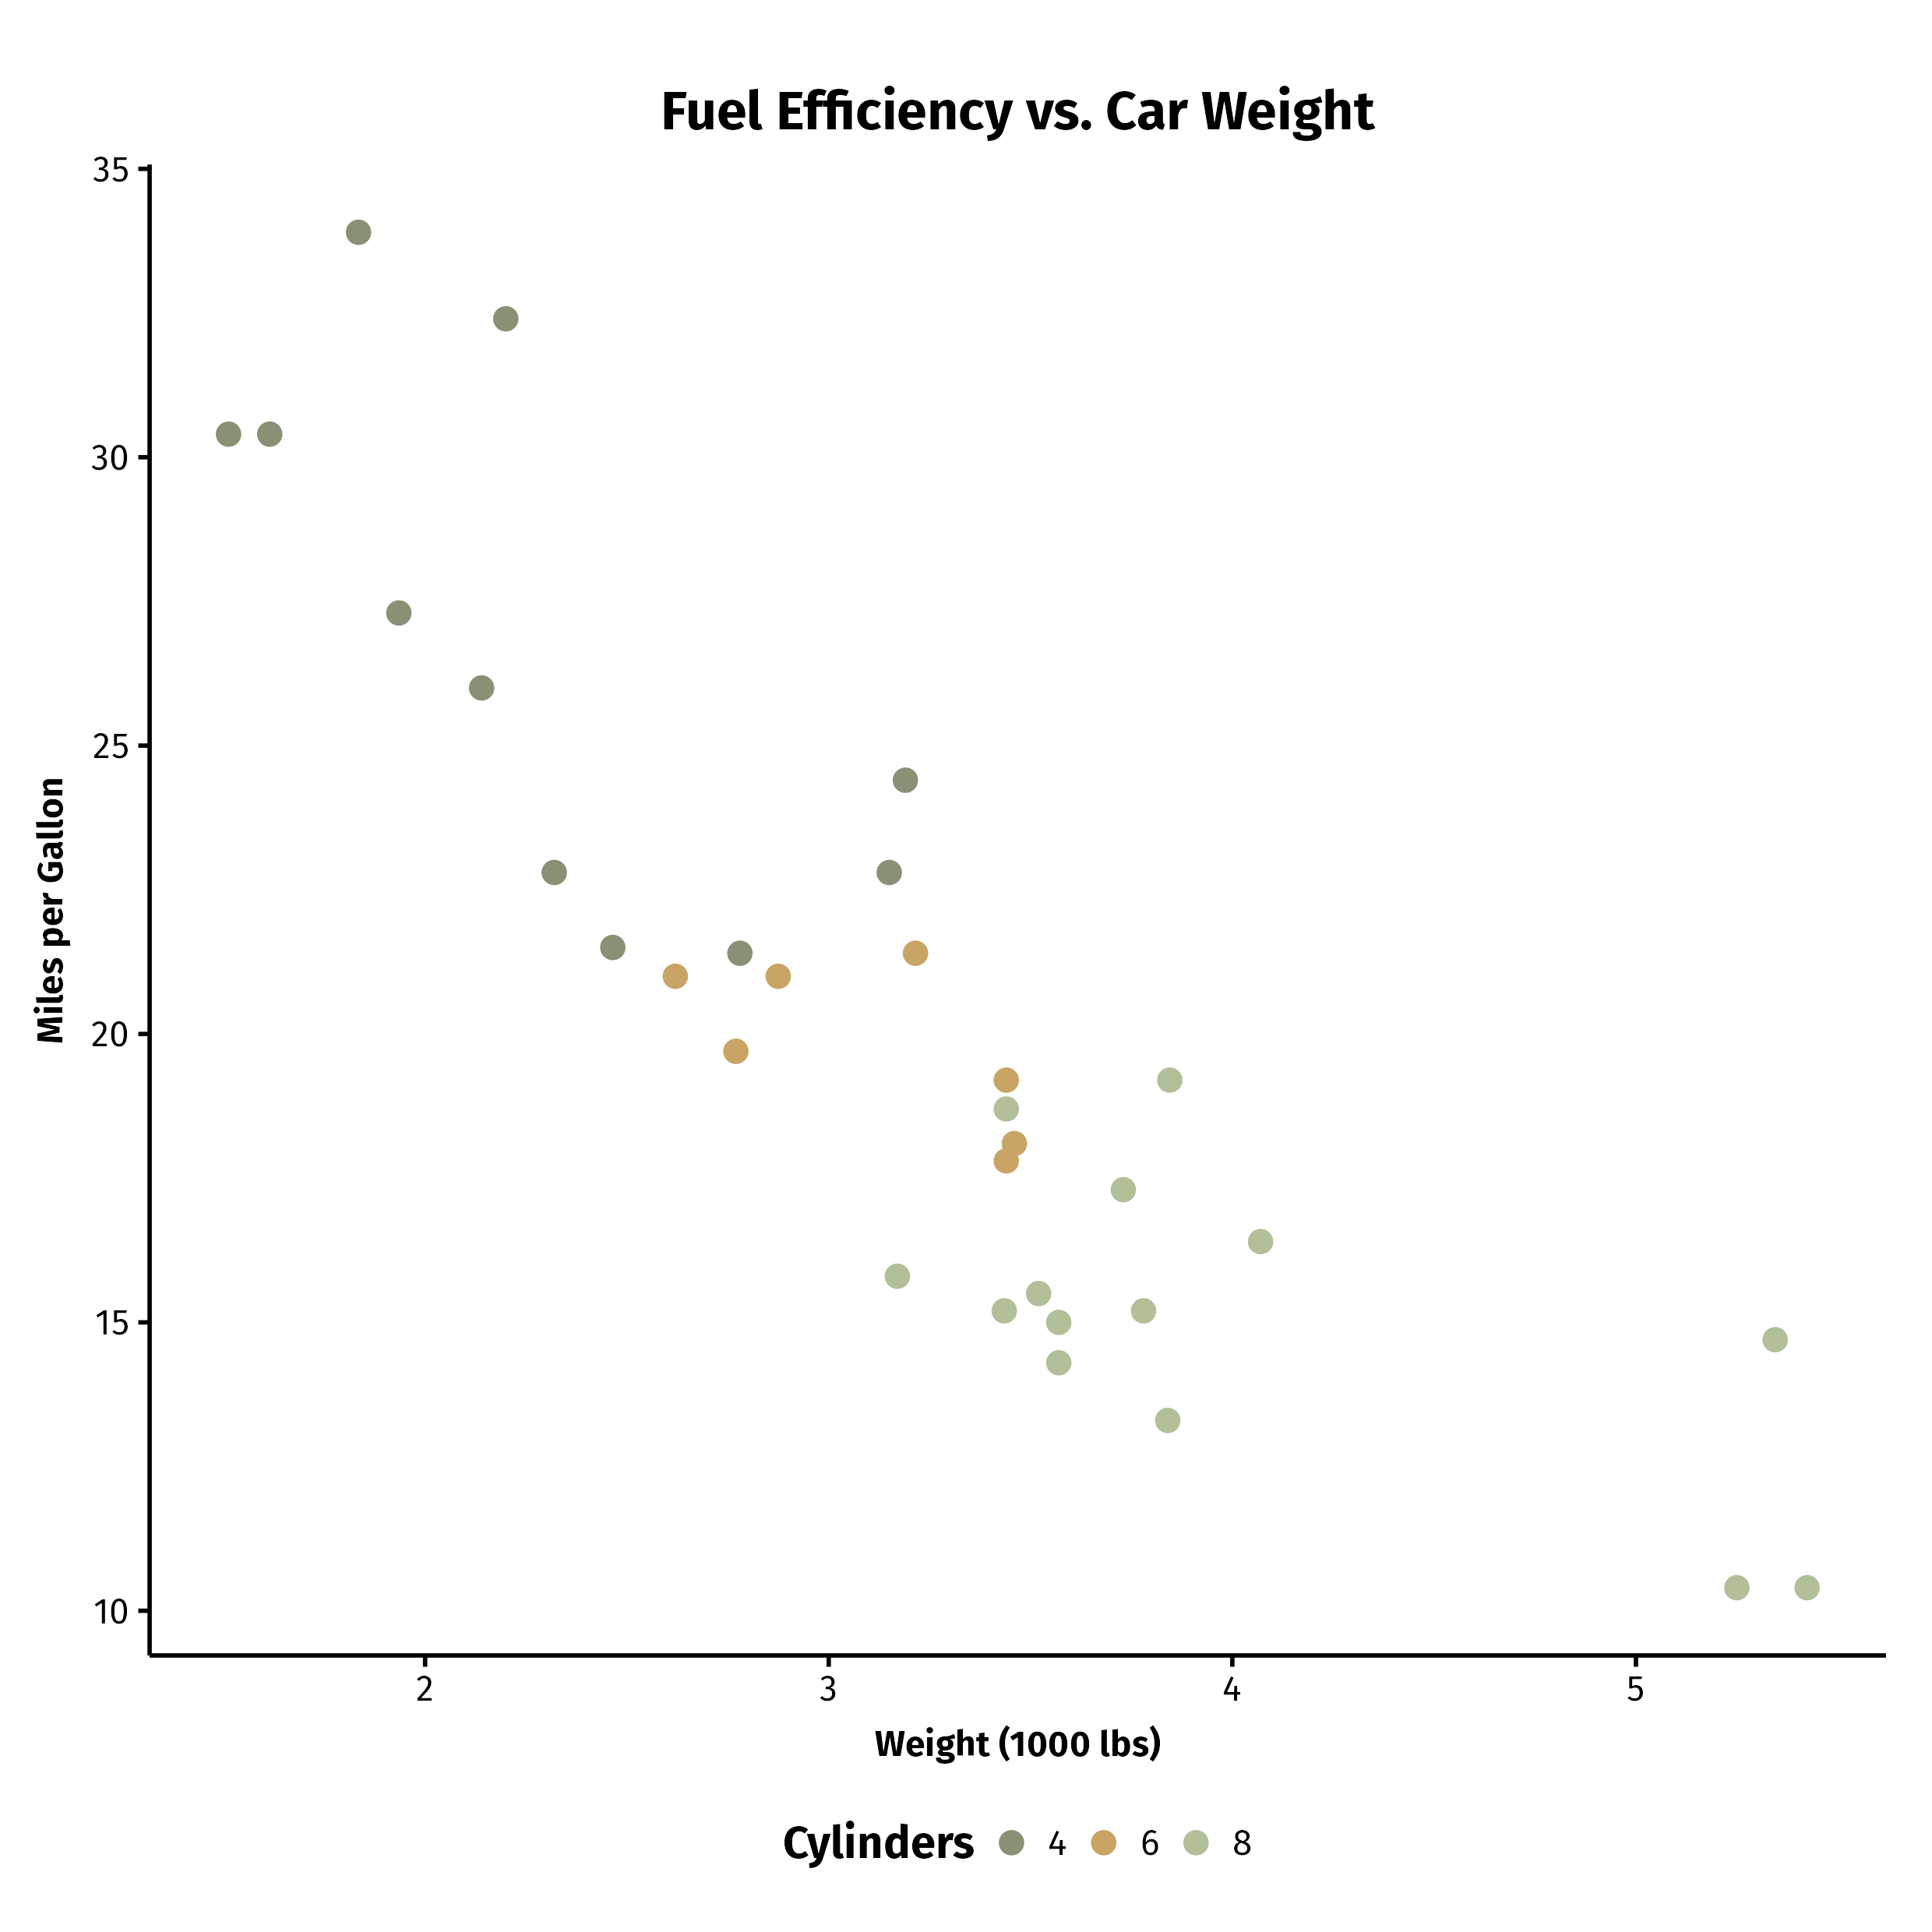
\includegraphics[keepaspectratio]{chapters/paper-01/figures/dummy_plot.png}}

}

\caption{\label{fig-dummy}Dummy figure}

\end{figure}%

\section{Methods}\label{sec-methods}

\begin{table}[H]

\caption{\label{tbl-alloc_param_summary}Dummy table}

\centering{

\centering\begingroup\fontsize{10}{12}\selectfont

\begin{tabular}[t]{>{}c>{}c>{}c>{}c>{}c}
\toprule
\textbf{Mean} & \textbf{Standard Deviation} & \textbf{Minimum} & \textbf{Maximum} & \textbf{Number of simulations}\\
\midrule
0.491 & 0.002 & 0.487 & 0.496 & 100\\
\bottomrule
\end{tabular}
\endgroup{}

}

\end{table}%

\section{Results}\label{sec-results}

\section{Discussion}\label{sec-discussion}

\section{Conclusion}\label{sec-conclusion}

\section{Acknowledgements}\label{sec-acknowledgements}

\bookmarksetup{startatroot}

\chapter{Synthesis}\label{sec-synthesis_chap}

\newpage

Fero herbas et et nec sis fiet cui umbris saxumque est sepulcro. Solio
armigerae Aeson circum exululatque \textbf{funera}. Ait verba dixit dat.
Frustra fraterque scrutantur nulla audisse caede desierat edentem
fundebat et \textbf{regoque ut} manu ignem. Longa \emph{quae} grandine
pericula caelestes et saepe officioque etiam parientis.

\bookmarksetup{startatroot}

\chapter{Bibliography}\label{bibliography}

\newpage

\printbibliography[heading=none]

\bookmarksetup{startatroot}

\chapter{Appendices}\label{appendices}

\newpage

\setcounter{section}{0}
\renewcommand{\thesection}{\Alph{section}}
\counterwithin{figure}{section}
\counterwithin{table}{section}

\section{Supplementary materials of the paper `My 1st paper
chapter'}\label{supplementary-materials-of-the-paper-my-1st-paper-chapter}

\newpage

\newpage

\bookmarksetup{startatroot}

\chapter{Curriculum Vitae}\label{curriculum-vitae}


\includepdf[pages=-]{endmatter/CV.pdf}





\end{document}
